\documentclass{report}

\begin{document}

\section{Introduzione}

\section{Meccanica}
% Composizione macchina
% Dimensionamento cinghie e motore
% Pneumatica

\chapter{Parte Meccanica}

\section{Descrizione macchina e motivazione dei componenti}

La parte meccanica, realizzata su Inventor, è stata divisa in 2 gruppi principali:

\begin{description}
\item \textbf{Trasporto}. La prima parte si occupa del trasporto del tubo mediante un asse lineare (corsa 300mm) che sfrutta una trasmissione a vite a ricircolo di sfere, comandata da un motore elettrico, per spostare un pistone pneumatico (1M1), dove alla sua estremità è montata una lamiera che con la sua elasticità garantisce la corretta aderenza al tubo, sfruttando tutta la forza del pistone. Il pistone è stato collegato al pattino dell’asse lineare mediante una lamiera e una piastra. Dalla parte opposta all’asse, troviamo una lamiera a forma di “V” che garantisce il corretto scorrimento del tubo fino alla parte di taglio, grazie all’utilizzo di una rulliera costruita con dei cuscinetti a sfera. 

Poco più a destra dell’asse lineare si colloca un altro pistone (2M1) fisso a telaio che si occupa di bloccare il tubo con la stessa logica del primo, contro un supporto in materiale tenero per non danneggiare l’oggetto da lavorare. 

All’estremità del telaio sono presenti delle lamiere che garantiscono il corretto ingresso ed uscita del tubo dalla parte di trasporto e dei sensori per controllare la posizione di quest’ultimo. Il telaio è stato realizzato mediante l’uso di tubolari quadrati in acciaio, dove sono stati fissati i supporti per le parti nominate in precedenza.

\item \textbf{Taglio ed espulsione}. La seconda parte si occupa del taglio e l’espulsione del tubo mediante l’uso di una sega circolare (d 300 mm) messa in moto da un motore elettrico monofase (P = 1,5 kW e rpm. max 2500), il tutto collegato con una trasmissione a cinghie piatte con rapporto di trasmissione i=0,5 che si occupa di moltiplicare i giri della puleggia operatrice per garantire un taglio ottimale, come consigliato da tabella. Il sottoassieme descritto è stato assemblato con un “telaietto” creato con dei tubolari quadrati in acciaio di piccole dimensioni per contenere il peso complessivo (motore, trasmissione, porta cuscinetto e lama) e vincolato ad un’estremità con 2 perni (che generano un effetto cerniera) che permettono la salita e la discesa di quest’ultimo, mediante un pistone a doppio effetto (3MX). Per trasformare lo spostamento lineare del pistone in angolare dovuto alla rotazione attorno ai perni sono stati montati dei perni a forcella, collocati tra una piastra fissa e la base del pistone e tra l’estremità dello stelo e il telaietto, garantendo una buona spinta senza considerevoli perdite di forze. 

Infine, troviamo l’espulsione del pezzo lavorato grazie all’utilizzo di un pistone pneumatico (4M1) dove all’estremità dello stelo è stata fissata una lamiera con delle prolunghe laterali che fanno scorrere il tubo su un piano d’appoggio (con la possibilità di essere allungato in base alla lunghezza del tubo desiderata) verso una caduta libera. Il telaio portante è stato realizzato mediante l’uso di tubolari quadrati in acciaio, dove sono stati fissati i supporti per le parti nominate in precedenza.

\end{description}

\section{Calcoli di progetto}
\subsection{Calcolo dei giri utili del motore}

I tubi da tagliare, utilizzati per il trasporto di fluidi possono esseri creati con 3 diversi materiali plastici:

\begin{description}
\item PVC (cloruro di polivinile) con	Rm = 55 MPa, mentre per il PVC-C Rm = 60 Mpa
\item PE (polietilene) 			Rm = 17 Mpa
\item PP (polipropilene) RM		Rm = 35 Mpa
\end{description}

PVC, PE e PP fanno parte della famiglia dei pannelli termoplastici (tabella V taglio consigliate) dove la V taglio consigliata si aggira tra i 50 e i 75 m/s e l’avanzamento tra 0,05 e 0,1 mm/z.

\begin{figure}[H] % per inserire l'immagine subito sotto il testo
    \centering
    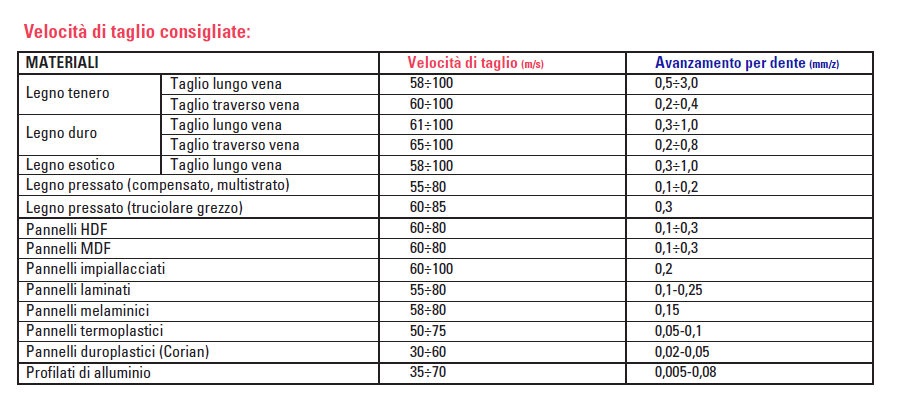
\includegraphics[width = 1\textwidth]{Tab Vtaglio lama.PNG}
    \caption{V taglio consigliate}
    \label{fig:my_label}
\end{figure}

Seguendo la linea nera (per materiali plastici) della tabella, assumiamo un D della lama circolare di 300 mm (inoltre utilizzata nella maggior parte dei casi, grazie al suo ottimo rapporto efficienza/ingombro).

\begin{figure}[H] % per inserire l'immagine subito sotto il testo
    \centering
    \includegraphics[width = 1\textwidth]{Vtaglio lama.PNG}
    \caption{Grafico V taglio consigliate}
    \label{fig:my_label}
\end{figure}

Conoscendo la V taglio richiesta dal materiale per essere tagliato possiamo calcolare il num. di giri generati dal motore, che successivamente verranno moltiplicati mediante una trasmissione a cinghie piatte.

Sappiamo che Vt = ω * r lama, di conseguenza rovesciando la formula ω = Vt / r, quindi:

\begin{description}
\item ω min = Vt / r = 50 [m/s] / 0,15 [m] = 334 rad/sec
\item ω max  = Vt / r = 75 [m/s] / 0,15 [m] = 500 rad/sec
\end{description}

Per una lettura più comoda converto la ω in rpm mediante la seguente formula: ω = (2*π*n)/60, di conseguenza rovesciando la formula n = (ω*60)/(2π), quindi:

\begin{description}
\item n min = (334*60)/(2π) = 3200 rpm (arrotondato per eccesso)
\item n max = (500*60)/(2π) = 4800 rpm (arrotondato per eccesso)
\end{description}

Conoscendo questi dati, con l’intenzione di utilizzare una trasmissione a cinghie piatte con un rapporto di trasmissione i = 0,5 (che moltiplica la velocità della puleggia operatrice del doppio rispetto a quella motrice) posso restringere il campo di ricerca del motore monofase a 2500 rpm massimi, che grazie alla trasmissione potrà raggiungere i 5000 rpm.

\subsection{Calcolo della forza di taglio}

La taglia del tubo da tagliare, nel nostro caso, ha le seguenti dimensioni:

\begin{description}

\item D = 104 mm
\item d  = 100 mm
\item A (sez. tubo) = 641 mm^2

\end{description}

Utilizzando il carico di rottura del materiale più resistente (PVC-C) con σ = 60 Mpa calcolo la sua τ, sapendo che τ = σ/ √3 e di conseguenza τ = k * (F/A) dove k per sezioni circolari è 4/3. Rovesciando la formula possiamo calcolare la F necessaria per tagliare il tubo.

\begin{description}

\item τ = 60/ √3 = 35 Mpa
\item τ = 1,34 * (F/A) dove F = (A*τ)/1,34 = 16.742,5 N

\end{description}

\subsection{Calcolo della potenza del motore}



\subsection{Dimensionamento della trasmissione}
Le cinghie sono organi flessibili impiegati nella trasmissione di potenza da una puleggia motrice a una condotta, montate su alberi disposti ad una certa distanza (interasse). Le cinghie possono appartenere a due gruppi distinti: cinghie di tipo convenzionale e cinghie sincrone.

Le cinghie di tipo convenzionale trasmettono il moto sfruttando l’aderenza (attrito) con il profilo esterno della puleggia. In questo caso possono verificarsi scorrimenti fra la cinghia e la puleggia durante il moto.
Le cinghie sincrone trasmettono il moto tramite l’ingranamento dei denti della cinghia con quelli della puleggia. Non sono soggette a scorrimento e necessitano di un precarico molto modesto.
Industrialmente sono usate cinghie piatte, trapezoidali e sincrone.

Per dimensionare una trasmissione partiamo dai dati del motore, forniti dal datasheet.

\begin{table}[H]
\centering
\begin{tabular}{|l|l|}
\hline
\multicolumn{2}{|c|}{\textbf{Dati motore}} \\ \hline
Potenza & 1,5 {[}kW{]} \\ \hline
Giri motore & 2500 {[}rpm{]} \\ \hline
D albero & 19 {[}mm{]} \\ \hline
\end{tabular}
\end{table}

Successivamente, una volta trovato il num. di giro che vogliamo sviluppare sull’operatrice (5000 rpm), calcolo il rapporto di trasmissione (i) e l’interasse (I) tra i due elementi rotanti in base alla dimensione delle mie pulegge, che assumo a piacere dalla serie di Renard R20 a partire da un diametro minimo di 40 mm.

Assumiamo D puleggia motrice 100 mm e di conseguenza (per rispettare il rapporto di trasmissione e la serie R20) 50 mm per il D dell’operatrice. Questa scelta è giustificata dagli ingombri in fase di modellazione 3D per tagliare correttamente il tubo senza urti.

Il calcolo dell’interasse dipende dal carico, nel nostro caso I >= 3-4 * D puleggia magg. per trasmissioni a carico variabile. Una volta rispettata questa condizione si può scegliere a piacimento la lunghezza in base alle esigenze (ingombri, etc…)


\begin{table}[H]
\centering
\begin{tabular}{|l|l|l|}
\hline
\multicolumn{2}{|c|}{\textbf{Dati Pulegge}} & \multicolumn{1}{c|}{\textbf{Formula}} \\ \hline
N giri motrice (n1) & 2500 {[}rpm{]} & Fornito dal motore \\ \hline
N giri operatrice (n2) & 5000 {[}rpm{]} & n1/i \\ \hline
Rapporto di trasmissione (i) & 0,5 & n1/n2 \\ \hline
\multicolumn{3}{|l|}{} \\ \hline
D puleggia motrice (D1) & 100 {[}mm{]} & Scelta personale rispettando R20 \\ \hline
D puleggia operatrice (D2) & 50 {[}mm{]} & D2 = D1 * i \\ \hline
Interasse (I) & 300 {[}mm{]} & I = 3 * D1 \\ \hline
\end{tabular}
\end{table}

Durante la progettazione di una trasmissione è importante consultare le tabelle unificate che forniscono dati di correzione in base ai materiali utilizzati per la realizzazione e il servizio che devono compiere.

Dati provenienti dalle tabelle del manuale di Meccanica:

\begin{table}[H]
\centering
\begin{tabular}{|l|l|l|}
\hline
\multicolumn{2}{|c|}{\textbf{Dati tabelle}} & \multicolumn{1}{c|}{\textbf{Provenienza dati}} \\ \hline
Fs & 1,2 & Tab. I.101 Fattore di servizio \\ \hline
Ft & 1 & Tab. I.102 Fattore correttivo \\ \hline
Fα & 1 & Tab. I.108 Coeff. correzione \\ \hline
P1 & 0,7 & Tab. I.106 P specifica (cinghia gomma-tessile) \\ \hline
\end{tabular}
\end{table}

\begin{description}

\item \textbf{Calcolo della potenza corretta}:
Pc = P*Fs*Ft [kW]

Dove P è la potenza erogata dal motore, Fs = 1,2 da tab. per macchine utensili che lavorano dalle 8 alle 10 ore al giorno ed Ft = 1 da tab. per condizioni normali.

Pc = 1,5*1,2*1 = 1,8 kW

\item \textbf{Calcolo della velocità periferica della puleggia minore}:

V = (π * D min * n D min)/60.000 [m/s] dove D min è D2 e n D min è n2

V = (π * 50 * 5000)/60.000 = 13,08 m/s

\item \textbf{Calcolo della lunghezza della cinghia}:

L = 2I + (π (D2+D1))/2 + ((D2-D1)^2)/4I [mm]

L = 837,6 mm che arrotondo a 840 mm per lasciare un po' di gioco prima di tendere e mollare la cinghia.


\item \textbf{Calcolo dell’angolo di avvolgimento (α)}:

α = 180 -57 * (D2-D1)/I [°]

α = 189,5 ° che mi servirà per trovare il valore di Fα da tab.

\item \textbf{Calcolo della larghezza della cinghia (a)}:

I principali materiali utilizzati per la costruzione di cinghie piatte sono:

    \begin{description}
    
    \item cuoio
    \item struttura composita di laminati plastici e gomme o resine
    \item struttura composita di gomme e tessili
    \item cotone, balata e altre fibre tessili vegetali
    \item gomma o materiali plastici (per alte velocità)
    
    \end{description}

Da questa informazione, possiamo calcolare la larghezza della cinghia, ricavando il valore P1 in base al materiale scelto (nel nostro caso gomma-tessile pesante in cotone a 4 tele) e la seguente formula:

a = Pc / (P1 * Fα) [cm]

a = 1,8 / (0,7*1) = 2,57 cm = 25,7 mm che unifico a 26 mm

La larghezza della cinghia corrisponde ai numeri della serie R40, a partire dal valore minimo di 16 mm.

\item \textbf{Calcolo dello spessore della cinghia (s)}:

Dalla seguente tabella ricavo lo spessore (s) della cinghia in base al materiale scelto in precedenza. In questo caso 6 mm.

\begin{figure}[H] % per inserire l'immagine subito sotto il testo
    \centering
    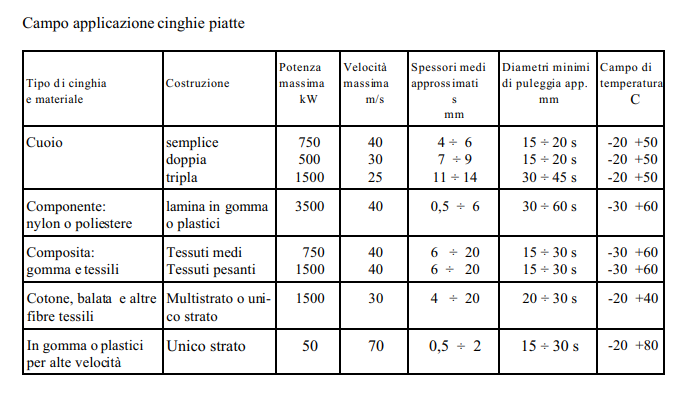
\includegraphics[width = 0.85\textwidth]{Cinghie piatte tabella.PNG}
    \caption{Parametri consigliati per vari tipi di cinghie}
    \label{fig:my_label}
\end{figure}

\item \textbf{Calcolo della larghezza della puleggia (b)}:

b = (1,1 ÷ 1,15) * a

b = 1,15 * 26 = 29,9 mm che arrotondo a 31 mm

\item \textbf{Calcolo della bombatura della puleggia (h)}:

Le pulegge per cinghie piatte vengono costruite con profilo esterno leggermente bombato per ottenere la stabilità della cinghia sulla corona. I materiali più indicati sono l’alluminio, per il peso contenuto, o la ghisa per piccole serie.

h = (0,5 ÷ 0,7%) * b

h = 0,6% * 31 = 0,19 mm


\end{description}


\section{Schema elettropneumatico}
\subsection{Scelta dei componenti}

Lo schema elettropneumatico è stato realizzato con i seguenti componenti:

\begin{figure}[H] % per inserire l'immagine subito sotto il testo
    \centering
    \includegraphics[width = 0.85\textwidth]{Impianto elettropneumatico.PNG}
    \caption{Schema Elettropneumatico}
    \label{fig:my_label}
\end{figure}

\begin{description}
\item \textbf{Compressore}: si occupa di accumulare e innalzare la pressione dell’aria all’interno del suo serbatoio per alimentare il circuito pneumatico.

\item \textbf{Gruppo trattamento aria}: composta da filtro di scarico manuale, un riduttore di pressione variabile, un manometro e una valvola di sicurezza (quasi sempre inclusa nei gruppi trattamento aria industriali per togliere aria al sistema in caso di emergenza).

\item \textbf{Pistone pinza mobile 1M1; Pistone pinza fissa 2M1; Pistone espulsore 4M1}: composti dalla stessa logica, tramite l'uso di:

    \begin{description}
    \item{1 pistone a singolo effetto con ritorno a molla (dove la sola corsa [50 mm] di andata è utile per svolgere il lavoro richiesto di bloccaggio ed espulsione).}
    \item{1 strozzatore. Si utilizza solamente uno strozzatore senza una o più valvole di non ritorno perché la regolazione della portata mediante strozzatura su ambedue i lati viene spesso applicata in cilindri a semplice effetto o in cilindri di piccole dimensioni che svolgono lavori “semplici”. Quest’aspetto inoltre va a vantaggio dei costi di realizzazione dell’impianto e della semplicità d’applicazione.}
     \item{1 valvola 3/2 normalmente chiusa comandata elettricamente nella fase di spinta e con ritorno a molla.}

    \end{description}

\item \textbf{Pistone sollevamento lama circolare}, composta da:

     \begin{description}
    \item{1 pistone a doppio effetto (corsa [100 mm]), che ha il compito di alzare ed abbassare il telaietto sul quale è montata la trasmissione (motore, cinghia, pulegge e lama).}
    \item{2 strozzatori in scarico per ottenere una buona regolazione della portata, entro certi limiti indipendenti dal carico applicato allo stelo, poiché viene guidato dal cuscino d’aria che si forma nella camera di scarico; agendo sulle viti di regolazione degli strozzatori si possono tarare separatamente le velocità delle due corse.}
     \item{1 valvola 5/3 a centri chiusi comandata elettricamente con ritorno a molla in ambedue i versi di commutazione per comandare il pistone a doppio effetto. La scelta di questa valvola è dovuta alla necessità di mantenere in posizione la lama (senza spostarsi in punti indesiderate, evitando danni all’oggetto da tagliare) in caso di arresto voluto o improvviso.}

    \end{description}

\item \textbf{Finecorsa dei pistoni}: Festo prevede l’utilizzo di sensori magneti che determinano la corsa dello stelo, montati direttamente sul cilindro.

\end{description}

\subsection{Riassunto qtà. componenti}

\begin{table}[H]
\centering
\begin{tabular}{|l|l|}
\hline
\multicolumn{1}{|c|}{\textbf{Componenti}} & \textbf{Qtà.} \\ \hline
Pistone sing. effetto & 3 \\ \hline
Pistone doppio effetto & 1 \\ \hline
Elettrovalvola 3/2 nc con ritorno a molla & 3 \\ \hline
Elettrovalvola 5/3 centri chiusi con ritorno a molla & 1 \\ \hline
Strozzatori & 5 \\ \hline
Valvole di non ritorno & 2 \\ \hline
Gruppo trattamento aria & 1 \\ \hline
Compressore & 1 \\ \hline
\end{tabular}
\end{table}



\section{Elettronica}
% PCB e quadro elettrico
% Dimensionamenti

\section{Programmazione}
% Schema a blocchi del sistema
% Spiegazione programma
% Ciclogramma

\section{Utilizzo della macchina}

\section{Sviluppi futuri}

\section{Crediti}


\end{document}